\defcatagory{Electricity}

\begin{question}%
  \qtitle{\termnoindex[charge]{Charge}\index{charge}\ldots}

  Quantity: $\text{\refterm{current}} \times \text{time}$~\hfill\point{1}

  Unit: \term{coulomb} = ampere second~\hfill\point{1}
\end{question}

\begin{question}%
  \qtitle{State what is meant by an electric \term{current}}\qpoint{1}

  flow of charge carriers~\hfill\point{1}
\end{question}

\begin{question}%
  \qtitle{Electric \refterm{current} is a flow of charge carriers. The \refterm{charge} on the carriers is quantised. Explain what is meant by \term{quantised}.}\qpoint{1}

  charge exists only in discrete amounts~\hfill\point{1}
\end{question}

\begin{question}%
  \qtitle{\termnoindex[potential difference]{Potential difference}\index{potential difference}\ldots}

  Quantity: $\frac{\text{\refterm{work} (done) or \refterm{energy} (transformed) (from electrical to other forms)}}{\refterm{charge}}$~\hfill\point{1}\vspace{0.5em}\\*
  \NOT Energy transferred \textit{by} unit charge / \SI{1}{C}.

  Unit: \term{volt} = $\frac{\text{\refterm{joule}}}{\text{\refterm{coulomb}}}$~\hfill\point{1}

  Not to be confused with \refterm{electromotive force}.
\end{question}

\begin{question}%
  \qtitle{Define \term{electromotive force} (e.m.f.) of a cell.}\qpoint{1}

  \refterm{energy} transformed from chemical to electrical per unit \refterm{charge}~\hfill\point{1}

  Not to be confused with \refterm{potential difference}.
\end{question}

\begin{question}%
  \label{q:ohm}%
  \qtitle{\termnoindex[resistance]{Resistance}\index{resistance}\ldots}

  Quantity: $\frac{\text{\refterm{potential difference}}}{\text{\refterm{current}}}$~\hfill\point{1}

  Unit: \term{ohm} = $\frac{\text{\refterm{volt}}}{\text{\refterm{ampere}}}$~\hfill\point{1}
\end{question}

\begin{question}%
  \qtitle{Define the \refterm{ohm}}\qpoint{1}

  $\frac{\text{\refterm{volt}}}{\text{\refterm{ampere}}}$~\hfill\point{1}\\*
  (See question~\ref{q:ohm}) \\*
  \NOT `unit of \refterm{resistance}'\vspace{0.5em}\\*
  \NOT `$\frac{\text{\refterm{potential difference}}}{\text{\refterm{current}}}$'
\end{question}

\begin{question}%
  \qtitle{Explain what is meant by an \term{electric field}}\qpoint{1}

  a region/space/area where a (stationary) \refterm{charge} experiences an (electric) \refterm{force}~\hfill\point{1}

  \NOT `Force per unit charge' etc.
\end{question}

\begin{question}%
  \qtitle{Define \term{electric field strength}}\qpoint{1}

  force \textbf{per} unit positive charge.~\hfill\point{1}

  See also: \refterm{electric field}
\end{question}

\clearpage
\begin{question}%
  \qtitle{On figure~\ref{fig:electric-field}, draw at least six field lines to represent the \refterm{electric field} between the plates.}\qpoint{1}

  \def\efbase{
    % \draw[help lines] (0, 0) grid[step=1] (7, 7);
    \path[fill] (1.45, 7) rectangle (1.55, 3) node [midway, anchor=center] (plateA) {};
    \path[fill] (4.95, 7) rectangle (5.05, 3) node [midway, anchor=center] (plateB) {};
  }

  Question:

  \hfill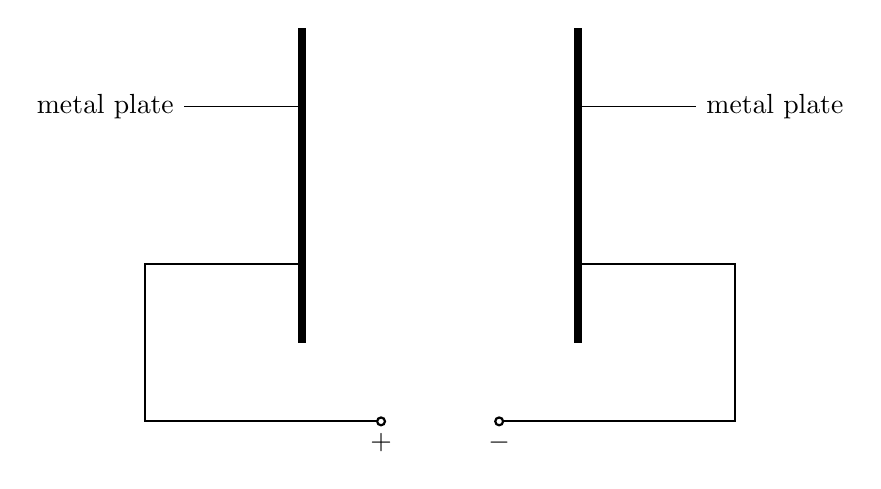
\begin{tikzpicture}[fill=black]
    \efbase
    \path[draw=black, thin] (plateA.center) ++(0, 1) -- ++(-1.5, 0) node[pos=1, left=0.25] {metal plate};
    \path[draw=black, thin] (plateB.center) ++(0, 1) -- ++(1.5, 0) node[pos=1, right=0.25] {metal plate};
    % wire for left plate
    \path[draw=black, thick] (plateA.center) ++(0, -1) -- ++(-2, 0) -- ++ (0, -2) -- ++(3, 0)
      node [shape=circle, inner sep=0.1em, draw=black, fill=white] {} node [pos=1, anchor=base, yshift=-1em] {$+$};
    % wire for right plate
    \path[draw=black, thick] (plateB.center) ++(0, -1) -- ++(2, 0) -- ++ (0, -2) -- ++(-3, 0)
      node [shape=circle, inner sep=0.1em, draw=black, fill=white] {} node [pos=1, anchor=base, yshift=-1em] {$-$};
  \end{tikzpicture}\hfill\null

  \refstepcounter{figure}\label{fig:electric-field}%
  \centerline{Figure~\thefigure: for question \ref{q\thequestion}}

  \begin{multicols}{3}
    Answer:\nopagebreak

    \hfill\begin{tikzpicture}[black]
      \efbase
      \foreach \y in {-1.5, -0.95, ..., 1.5} {\path[draw] ($(plateA)+(0, \y)$) -- ($(plateB) + (0, \y)$) node [midway, anchor=center] {$>$};};
    \end{tikzpicture}\hfill\null

    \NOT\nopagebreak

    \hfill\begin{tikzpicture}[not]
      \efbase
      \foreach \y in {-1.5, -1.4, -1.2, -0.8, 0, 1.6} {\path[draw] ($(plateA)+(0, \y)$) -- ($(plateB) + (0, \y)$) node [midway, anchor=center] {$>$};};
    \end{tikzpicture}\hfill\null

    \NOT\nopagebreak

    \hfill\begin{tikzpicture}[not]
      \efbase
      \foreach \y in {-1.5, -0.95, ..., 1.5} {\path[draw] ($(plateA)+(0, \y)$) -- ($(plateB) + (0, \y)$);};
    \end{tikzpicture}\hfill\null

    \NOT\nopagebreak

    \hfill\begin{tikzpicture}[not]
      \efbase
      \foreach \y in {-1.5, -0.95, ..., 1.5} {\path[draw] ($(plateA)+(0, \y)$) -- ($(plateB) + (0, \y)$) node [midway, anchor=center] {$<$};};
    \end{tikzpicture}\hfill\null

    \NOT\nopagebreak

    \hfill\begin{tikzpicture}[not]
      \efbase
      \foreach \y in {-1.5, -0.95, ..., 1.5} {\path[draw, transform canvas={yslant=0.3, yshift=-2.4em}] ($(plateA)+(0, \y)$) -- ($(plateB) + (0, \y)$) node [midway, anchor=center] {$>$};};
    \end{tikzpicture}\hfill\null

    \NOT\nopagebreak

    \hfill\begin{tikzpicture}[not]
      \efbase
      \foreach \y in {-1.5, -0.95, ..., 1.5} {\path[draw, style={
        decorate, decoration={random steps,segment length=6pt,amplitude=1.5pt}
      }] ($(plateA)+(0, \y)$) -- ($(plateB) + (0, \y)$) node [midway, anchor=center] {$>$};};
    \end{tikzpicture}\hfill\null\nopagebreak

    i.e. use ruler.
  \end{multicols}
\end{question}

\begin{question}%
  \qtitle{Explain why the calculation of the \refterm{force} on a electron in an \refterm{electric field} does not need to include the gravitational effects on the electron.}\qpoint{1}

  electric force is way bigger than gravitational force (on electron)/weight~\hfill\point{1}\\*
  \OR something about acceleration being way bigger.

  \NOT gravitational force is negligible
\end{question}

\def\ivaxisbase{
  \path[draw, help lines, opacity=0.5] (-3, -3) grid[step=0.5] (3, 3);
  \path[thick, draw, ->] (0, -3.5) -- (0, 3.5) node[above=0.5em] {$I$};
  \path[thick, draw, ->] (-3.5, 0) -- (3.5, 0) node[above=0.5em] {$V$};
}
\begin{figure}
  \figureruletop

  \begin{multicols}{2}
    \centering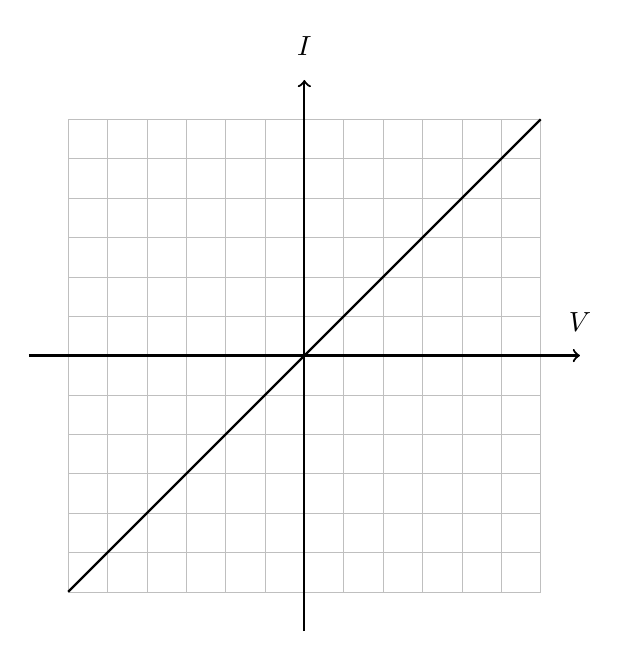
\begin{tikzpicture}
      \ivaxisbase
      \path[draw, thick] (-3, -3) -- (3, 3);
    \end{tikzpicture}\nopagebreak

    \reftermnoindex[resistor]{Metallic}\filbreak

    \centering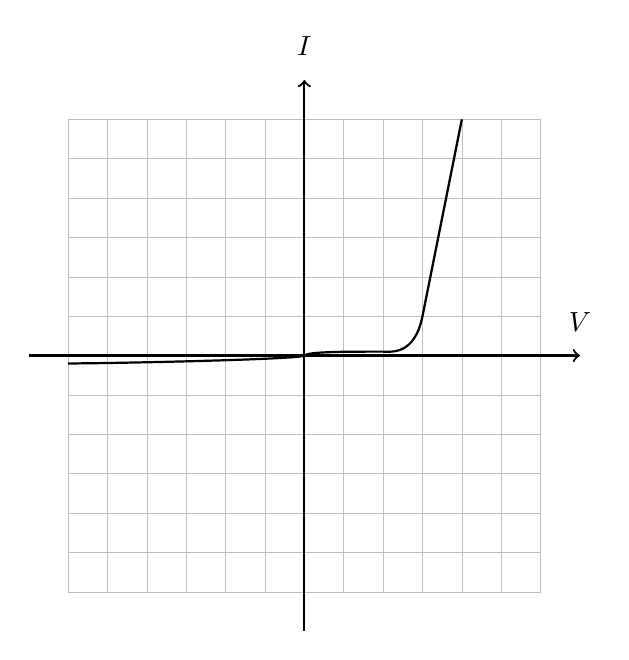
\begin{tikzpicture}
      \ivaxisbase
      \path[draw, thick] (-3, -0.1) .. controls (-2.5, -0.1) and (-0.05, -0.05) .. (0, 0) .. controls (0.05, 0.05) and (0.5, 0.05) .. (1, 0.05) .. controls +(0.1, 0) and (1.4, 0) .. (1.5, 0.5) -- (2, 3);
    \end{tikzpicture}\nopagebreak

    \reftermnoindex[diode]{Diode}\index{diode}\filbreak

  \end{multicols}

  \centering\begin{tikzpicture}
    \ivaxisbase
    \path[draw, thick] (-3, -3) .. controls (-0.5, -2.5) and (0.5, 2.5) .. (3, 3) node[pos=1, anchor=center] (tip) {};
    \path[<-, draw, thick] (tip) .. controls +(0, 1em) and ($(tip) + (0.5em, 1.5em)$) .. ($(tip) + (1em, 1.5em)$)
      node[pos=1, label={right:\NOT zero gradient at tip}]{};
  \end{tikzpicture}\nopagebreak

  \centering\reftermnoindex[filament lamp]{Filament lamp}\index{filament lamp}\filbreak

  \caption{\term{I-V graph} for question~\ref{q:iv1},~\ref{q:iv2}~and~\ref{q:iv3}}
  \label{fig:iv}

  \figureruletbottom
\end{figure}

\begin{question}%
  \label{q:iv1}%
  \qtitle{Describe the I-V characteristic of a metallic conductor at constant temperature}\qpoint{1}

  straight line \textbf{through the origin}~\hfill\point{1}

  See figure~\ref{fig:iv}
\end{question}

\begin{question}%
  \label{q:iv2}%
  \qtitle{Describe the I-V characteristic of a semiconductor \refterm{diode}}\qpoint{2}

  zero current for one direction up to zero or a few tenths of volt in another direction~\hfill\point{1}\\*
  straight line positive gradient/increasing gradient (after that)~\hfill\point{1}

  See figure~\ref{fig:iv}
\end{question}

\begin{question}%
  \label{q:iv3}%
  \qtitle{Use figure~\ref{fig:iv} to describe the variation of the resistance of the \refterm{diode} between $V = \SI{-0.5}{V}$ and $V = \SI{0.8}{V}$.}\qpoint{2}

  very high/infinite \refterm{resistance} for negative \reftermnoindex[potential difference]{voltages} up to about \SI{0.6}{V} / some number in graph given
  in question.~\hfill\point{1}\\*
  resistance decreases from \textit{<that voltage>}~\hfill\point{1}

  \NOT zero \refterm{current} means zero \refterm{resistance}\\*
  The gradient of the graph is \NOT \refterm{resistance}.
\end{question}

\begin{question}%
  \qtitle{State Kirchhoff's $n$th law\ldots}

  \begin{itemize}
    \item \termnoindex[kirchhoff 1st]{$n = 1$}\index{Kirchhoff's first law}:\qpoint{1}

      sum of currents into a junction = sum of currents out of junction~\hfill\point{1}

    \item \termnoindex[kirchhoff 2nd]{$n = 2$}\index{Kirchhoff's second law}:\qpoint{2}

      \textbf{total/sum} of electromotive forces/e.m.f.s = \textbf{total/sum} of potential differences/p.d.s~\hfill\point{1}\\*
      around a loop/(closed) circuit~\hfill\point{1}

    \item There is no third law. (Although there is \reftermnoindex[newton 3rd]{a third law by Newton}.)
  \end{itemize}
\end{question}

\begin{question}%
  \qtitle{\refterm[kirchhoff 1st]{Kirchhoff's first law} is linked to the conservation of a certain quantity. State this quantity.}\qpoint{1}

  \refterm{charge}~\hfill\point{1}\\*
  \NOT \refterm{current}
\end{question}

\begin{question}%
  \qtitle{Sketch the temperature characteristic of a (NTC) \refterm{thermistor}}\qpoint{2}

  \def\axisbase{
    \path[draw, thick, ->] (0, -0.1) -- (0, 5) node[pos=0, below] {$0$} node[pos=0.75, left=1em] {\refterm{resistance}};
    \path[draw, thick, ->] (-0.1, 0) -- (10, 0) node[pos=1, below left, shift={(0, -0.5)}] {\refterm{temperature} $/ \SI{}{\degree C}$};
    \path[draw] (6.5, 0) -- (6.5, -0.1) node[below] {100};
  }

  Answer:\nopagebreak

  \begin{tikzpicture}
    \axisbase
    \path[draw, thin] (0, 4) .. controls (0.5, 2) and (5, 1.3) .. (10, 1);
  \end{tikzpicture}\filbreak

  \NOT\nopagebreak

  \begin{tikzpicture}[draw=not, not]
    \axisbase
    \path[draw, thin] (0, 4) .. controls (0.5, 2) and (5, 0.3) .. (10, 0);
  \end{tikzpicture}\filbreak
\end{question}
